% Options for packages loaded elsewhere
\PassOptionsToPackage{unicode}{hyperref}
\PassOptionsToPackage{hyphens}{url}
\PassOptionsToPackage{dvipsnames,svgnames*,x11names*}{xcolor}
%
\documentclass[12pt,
  a4paper,
  landscape]{article}
\usepackage{lmodern}
\usepackage{amsmath}
\usepackage{ifxetex,ifluatex}
\ifnum 0\ifxetex 1\fi\ifluatex 1\fi=0 % if pdftex
  \usepackage[T1]{fontenc}
  \usepackage[utf8]{inputenc}
  \usepackage{textcomp} % provide euro and other symbols
  \usepackage{amssymb}
\else % if luatex or xetex
  \usepackage{unicode-math}
  \defaultfontfeatures{Scale=MatchLowercase}
  \defaultfontfeatures[\rmfamily]{Ligatures=TeX,Scale=1}
\setmainfont{Atkinson Hyperlegible}
\setsansfont{Atkinson Hyperlegible}
  \setmonofont[]{Fira Code}
\fi
% Use upquote if available, for straight quotes in verbatim environments
\IfFileExists{upquote.sty}{\usepackage{upquote}}{}
\IfFileExists{microtype.sty}{% use microtype if available
  \usepackage[]{microtype}
  \UseMicrotypeSet[protrusion]{basicmath} % disable protrusion for tt fonts
}{}
\makeatletter
\@ifundefined{KOMAClassName}{% if non-KOMA class
  \IfFileExists{parskip.sty}{%
    \usepackage{parskip}
  }{% else
    \setlength{\parindent}{0pt}
    \setlength{\parskip}{6pt plus 2pt minus 1pt}}
}{% if KOMA class
  \KOMAoptions{parskip=half}}
\makeatother
\usepackage[dvipsnames]{xcolor}
\IfFileExists{xurl.sty}{\usepackage{xurl}}{} % add URL line breaks if available
\IfFileExists{bookmark.sty}{\usepackage{bookmark}}{\usepackage{hyperref}}
\hypersetup{
  pdftitle={Lecture 01:   Replace it!},
  pdfauthor={Dr.~Gordon Wright},
  colorlinks=true,
  linkcolor=blue,
  filecolor=Maroon,
  citecolor=Blue,
  urlcolor=Blue,
  pdfcreator={LaTeX via pandoc}}
\urlstyle{same} % disable monospaced font for URLs
\usepackage[a4paper, margin=1in]{geometry}

\usepackage{longtable,booktabs}
\usepackage{calc} % for calculating minipage widths
% Correct order of tables after \paragraph or \subparagraph
\usepackage{etoolbox}
\makeatletter
\patchcmd\longtable{\par}{\if@noskipsec\mbox{}\fi\par}{}{}
\makeatother
% Allow footnotes in longtable head/foot
\IfFileExists{footnotehyper.sty}{\usepackage{footnotehyper}}{\usepackage{footnote}}
\makesavenoteenv{longtable}
\usepackage{graphicx}
\makeatletter
\def\maxwidth{\ifdim\Gin@nat@width>\linewidth\linewidth\else\Gin@nat@width\fi}
\def\maxheight{\ifdim\Gin@nat@height>\textheight\textheight\else\Gin@nat@height\fi}
\makeatother
% Scale images if necessary, so that they will not overflow the page
% margins by default, and it is still possible to overwrite the defaults
% using explicit options in \includegraphics[width, height, ...]{}
\setkeys{Gin}{width=\maxwidth,height=\maxheight,keepaspectratio}
% Set default figure placement to htbp
\makeatletter
\def\fps@figure{htbp}
\makeatother
\setlength{\emergencystretch}{3em} % prevent overfull lines
\providecommand{\tightlist}{%
  \setlength{\itemsep}{0pt}\setlength{\parskip}{0pt}}
\setcounter{secnumdepth}{-\maxdimen} % remove section numbering
% Make \paragraph and \subparagraph free-standing
\ifx\paragraph\undefined\else
  \let\oldparagraph\paragraph
  \renewcommand{\paragraph}[1]{\oldparagraph{#1}\mbox{}}
\fi
\ifx\subparagraph\undefined\else
  \let\oldsubparagraph\subparagraph
  \renewcommand{\subparagraph}[1]{\oldsubparagraph{#1}\mbox{}}
\fi
\usepackage{fancyhdr}
\pagestyle{fancy}
\fancyhead[L]{today}
\fancyhead[C]{Central}
\fancyhead[R]{Right}
\fancyfoot[R]{PS51234X - Research Methods}
\fancyfoot[C]{\thepage}
\renewcommand{\headrulewidth}{0.4pt}
\renewcommand{\footrulewidth}{0.4pt}
\makeatletter
\@ifpackageloaded{tcolorbox}{}{\usepackage[skins,breakable]{tcolorbox}}
\@ifpackageloaded{fontawesome5}{}{\usepackage{fontawesome5}}
\definecolor{quarto-callout-color}{HTML}{909090}
\definecolor{quarto-callout-note-color}{HTML}{0758E5}
\definecolor{quarto-callout-important-color}{HTML}{CC1914}
\definecolor{quarto-callout-warning-color}{HTML}{EB9113}
\definecolor{quarto-callout-tip-color}{HTML}{00A047}
\definecolor{quarto-callout-caution-color}{HTML}{FC5300}
\definecolor{quarto-callout-color-frame}{HTML}{acacac}
\definecolor{quarto-callout-note-color-frame}{HTML}{4582ec}
\definecolor{quarto-callout-important-color-frame}{HTML}{d9534f}
\definecolor{quarto-callout-warning-color-frame}{HTML}{f0ad4e}
\definecolor{quarto-callout-tip-color-frame}{HTML}{02b875}
\definecolor{quarto-callout-caution-color-frame}{HTML}{fd7e14}
\makeatother
\makeatletter
\makeatother
\makeatletter
\makeatother
\makeatletter
\@ifpackageloaded{caption}{}{\usepackage{caption}}
\AtBeginDocument{%
\ifdefined\contentsname
  \renewcommand*\contentsname{Table of contents}
\else
  \newcommand\contentsname{Table of contents}
\fi
\ifdefined\listfigurename
  \renewcommand*\listfigurename{List of Figures}
\else
  \newcommand\listfigurename{List of Figures}
\fi
\ifdefined\listtablename
  \renewcommand*\listtablename{List of Tables}
\else
  \newcommand\listtablename{List of Tables}
\fi
\ifdefined\figurename
  \renewcommand*\figurename{Figure}
\else
  \newcommand\figurename{Figure}
\fi
\ifdefined\tablename
  \renewcommand*\tablename{Table}
\else
  \newcommand\tablename{Table}
\fi
}
\@ifpackageloaded{float}{}{\usepackage{float}}
\floatstyle{ruled}
\@ifundefined{c@chapter}{\newfloat{codelisting}{h}{lop}}{\newfloat{codelisting}{h}{lop}[chapter]}
\floatname{codelisting}{Listing}
\newcommand*\listoflistings{\listof{codelisting}{List of Listings}}
\makeatother
\makeatletter
\@ifpackageloaded{caption}{}{\usepackage{caption}}
\@ifpackageloaded{subcaption}{}{\usepackage{subcaption}}
\makeatother
\makeatletter
\@ifpackageloaded{tcolorbox}{}{\usepackage[skins,breakable]{tcolorbox}}
\makeatother
\makeatletter
\@ifundefined{shadecolor}{\definecolor{shadecolor}{rgb}{.97, .97, .97}}
\makeatother
\makeatletter
\makeatother
\makeatletter
\makeatother
\makeatletter
\@ifpackageloaded{fontawesome5}{}{\usepackage{fontawesome5}}
\makeatother
\ifluatex
  \usepackage{selnolig}  % disable illegal ligatures
\fi
\newlength{\cslhangindent}
\setlength{\cslhangindent}{1.5em}
\newlength{\csllabelwidth}
\setlength{\csllabelwidth}{3em}
\newenvironment{CSLReferences}[2] % #1 hanging-ident, #2 entry spacing
 {% don't indent paragraphs
  \setlength{\parindent}{0pt}
  % turn on hanging indent if param 1 is 1
  \ifodd #1 \everypar{\setlength{\hangindent}{\cslhangindent}}\ignorespaces\fi
  % set entry spacing
  \ifnum #2 > 0
  \setlength{\parskip}{#2\baselineskip}
  \fi
 }%
 {}
\usepackage{calc}
\newcommand{\CSLBlock}[1]{#1\hfill\break}
\newcommand{\CSLLeftMargin}[1]{\parbox[t]{\csllabelwidth}{#1}}
\newcommand{\CSLRightInline}[1]{\parbox[t]{\linewidth - \csllabelwidth}{#1}\break}
\newcommand{\CSLIndent}[1]{\hspace{\cslhangindent}#1}

\title{\textbf{Lecture 01: Replace it!}}
\usepackage{etoolbox}
\makeatletter
\providecommand{\subtitle}[1]{% add subtitle to \maketitle
  \apptocmd{\@title}{\par {\large #1 \par}}{}{}
}
\makeatother
\subtitle{This is a meaningful subtitle}
\author{Dr.~Gordon Wright}
\date{October 2, 2023}

% my preamble additions =============================================================

% left justify text with ragged right edge =====================================
\usepackage[document]{ragged2e}

% page numbering ===============================================================
\usepackage{fancyhdr}
\pagestyle{fancy}
\fancyhf{}
\renewcommand{\headrulewidth}{0pt}
\fancyfoot[L]{\footnotesize\textcolor{gray}{PS52007D}}
\fancyfoot[C]{\footnotesize\textcolor{gray}{Lecture 01: Replace it!}}
\fancyfoot[R]{\footnotesize\textcolor{gray}{\thepage}}

% change default spacing before each new paragraph (sets as text height) =======
\setlength\parskip{1em plus 0.1em minus 0.2em}

% set formatting for section and subsection headings ===========================
% adding a period after section numbering
% \usepackage{titlesec}
% \titlelabel{\thetitle.\quad}
% comment/uncomment the next line to insert a page break before each new H1
\let\oldsection\section
\renewcommand\section{\clearpage\oldsection}

% changing options for table/figure captions ===================================
% uncomment the below lines to just number figures/tables sequentially
% throughout entire document
% \renewcommand{\thetable}{\thesection.\arabic{table}}
% \renewcommand{\thefigure}{\thesection.\arabic{figure}}

\usepackage[labelfont=it,textfont=it,singlelinecheck=off,justification=raggedright,labelsep=period]{caption}

% resets table/figure counters within each section/subsection ==================
% \usepackage{chngcntr}
% \counterwithin*{table}{section}
%\counterwithin*{table}{subsection}
% \counterwithin*{figure}{section}
%\counterwithin*{figure}{subsection}

\usepackage{tcolorbox}

\definecolor{cosmiclatte}{RGB}{255, 248, 231}
\definecolor{justoffwhite}{RGB}{255, 254, 250}

%\definecolor{notes-bg}{RGB}{254, 250, 233}
%\definecolor{notes-frame}{RGB}{222, 217, 193}

%\definecolor{Questions-bg}{RGB}{236, 239, 244}
%\definecolor{Questions-frame}{RGB}{236, 239, 244}

\definecolor{notes-bg}{RGB}{244, 247, 252}
\definecolor{notes-frame}{RGB}{233, 235, 238}
\definecolor{notes-text}{RGB}{47, 54, 61}

\definecolor{slide-titles}{RGB}{47, 54, 61}

\usepackage{pagecolor}
\usepackage{afterpage}

\renewcommand{\baselinestretch}{1.5}

% resize headings =============================

\makeatletter

\renewcommand{\section}{\@startsection
{section}%                   % the name
{1}%                         % the level
{\z@}%                       % the indent / 0mm
{3\baselineskip}%            % the before skip / -3.5ex \@plus -1ex \@minus -.2ex
{3\baselineskip}%          % the after skip / 2.3ex \@plus .2ex
{\sffamily\huge\bfseries}} % the style

\renewcommand{\subsection}{\@startsection
{subsection}%                   % the name
{2}%                         % the level
{\z@}%                       % the indent / 0mm
{3\baselineskip}%            % the before skip / -3.5ex \@plus -1ex \@minus -.2ex
{.75\baselineskip}%          % the after skip / 2.3ex \@plus .2ex
{\sffamily\Large\bfseries\textcolor{slide-titles}}} % the style

\renewcommand{\subsubsection}{\@startsection
{subsubsection}%                   % the name
{3}%                         % the level
{\z@}%                       % the indent / 0mm
{3\baselineskip}%            % the before skip / -3.5ex \@plus -1ex \@minus -.2ex
{.75\baselineskip}%          % the after skip / 2.3ex \@plus .2ex
{\large\bfseries}} % the style

\makeatother

\usepackage[export]{adjustbox}

% ===================================================================================

\begin{document}


      % \maketitle
    \begin{center}
    \vspace*{5cm}
    {\Huge\bfseries Lecture 01: Replace it!}\\
          \vfill
      {\large\bfseries PS52007D}
        \end{center}
    % turn off page numbering for titlepage
    \thispagestyle{empty}
        \newpage
  
\ifdefined\Shaded\renewenvironment{Shaded}{\begin{tcolorbox}[enhanced, frame hidden, boxrule=0pt, interior hidden, sharp corners, breakable, borderline west={3pt}{0pt}{shadecolor}]}{\end{tcolorbox}}\fi





\hypertarget{show-attendance-qr-code}{%
\section{Show Attendance QR Code}\label{show-attendance-qr-code}}

\hypertarget{heading-1---section-head}{%
\section{Heading 1 - Section Head}\label{heading-1---section-head}}

This is a subtitle to the section header

\hypertarget{heading-2---new-slide-title}{%
\subsection{Heading 2 - new slide
title}\label{heading-2---new-slide-title}}

Heading 2 copy

\hypertarget{heading-3---italic-emphasis}{%
\subsubsection{Heading 3 - italic
emphasis}\label{heading-3---italic-emphasis}}

\hypertarget{spans-for-text-accentuation---available-in-source-mode}{%
\subsection{Spans for text accentuation - available in source
mode}\label{spans-for-text-accentuation---available-in-source-mode}}

{.shout} accent3(red) 1.5em and Bold

{.alert} accent3(red) no change to font size

{.fg} {.bg}

{.button} accent1 whitetext button for link

{.button-success}

{.takeaway}

{.highlight}

\hypertarget{citations}{%
\subsection{Citations}\label{citations}}

Wright et al. (2012)

Cohen (1992) In text citation \texttt{@Cohen1992}

(Cohen, 1992) not in-text citation `(Cohen, 1992)

just type `@` and a search box comes up for your Zotero library or a
.bib file associated with the project

\hypertarget{imagecontent-2-column}{%
\subsection{Image\textbar content 2
column}\label{imagecontent-2-column}}

Slide with image and commentary in two columns and some explanatory text
above

text text text text text text text text text text text text

text text text text text text text text text text text text

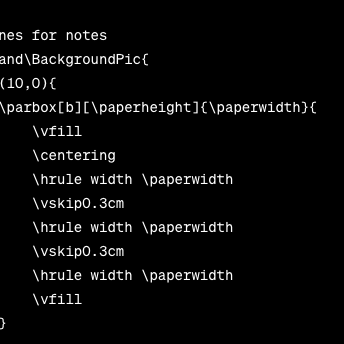
\includegraphics{images/TestImage.png}

Here is some text

\begin{itemize}
\item
  Bullet 1
\item
  Bullet 2
\item
  Bullet 3
\end{itemize}

\hypertarget{callouts}{%
\subsection{Callouts}\label{callouts}}

\hypertarget{note-callouts}{%
\subsection{Note Callouts}\label{note-callouts}}

\begin{tcolorbox}[enhanced jigsaw, titlerule=0mm, colbacktitle=quarto-callout-note-color!10!white, arc=.35mm, colframe=quarto-callout-note-color-frame, colback=white, toptitle=1mm, breakable, bottomrule=.15mm, left=2mm, toprule=.15mm, opacitybacktitle=0.6, rightrule=.15mm, coltitle=black, bottomtitle=1mm, title=\textcolor{quarto-callout-note-color}{\faInfo}\hspace{0.5em}{Note default}, leftrule=.75mm, opacityback=0]

content

\end{tcolorbox}

\begin{tcolorbox}[enhanced jigsaw, left=2mm, toprule=.15mm, arc=.35mm, leftrule=.75mm, rightrule=.15mm, colframe=quarto-callout-note-color-frame, colback=white, opacityback=0, breakable, bottomrule=.15mm]
\begin{minipage}[t]{5.5mm}
\textcolor{quarto-callout-note-color}{\faInfo}
\end{minipage}%
\begin{minipage}[t]{\textwidth - 5.5mm}

\textbf{Note simple}\vspace{2mm}

content

\end{minipage}%
\end{tcolorbox}

\begin{tcolorbox}[enhanced jigsaw, left=2mm, toprule=.15mm, arc=.35mm, leftrule=.75mm, rightrule=.15mm, colframe=quarto-callout-note-color-frame, colback=white, opacityback=0, breakable, bottomrule=.15mm]

\textbf{Note minimal}\vspace{2mm}

content

\end{tcolorbox}

\hypertarget{icons-by-fontawesome}{%
\subsection{Icons by FontAwesome}\label{icons-by-fontawesome}}

These are cool \faIcon{user} but they do need a full render e.g.
\texttt{\$\ quarto\ render} in order to be seen.

They can also be used in pdfs

\begin{longtable}[]{@{}
  >{\raggedright\arraybackslash}p{(\columnwidth - 2\tabcolsep) * \real{0.4722}}
  >{\centering\arraybackslash}p{(\columnwidth - 2\tabcolsep) * \real{0.5278}}@{}}
\caption{Fontawesome}\tabularnewline
\toprule\noalign{}
\begin{minipage}[b]{\linewidth}\raggedright
input
\end{minipage} & \begin{minipage}[b]{\linewidth}\centering
output
\end{minipage} \\
\midrule\noalign{}
\endfirsthead
\toprule\noalign{}
\begin{minipage}[b]{\linewidth}\raggedright
input
\end{minipage} & \begin{minipage}[b]{\linewidth}\centering
output
\end{minipage} \\
\midrule\noalign{}
\endhead
\bottomrule\noalign{}
\endlastfoot
\texttt{\{\{\textless{}\ fa\ binoculars\ \textgreater{}\}\}} &
\faIcon{binoculars} Prepare \\
\texttt{\{\{\textless{}\ fa\ chalkboard-teacher\ \textgreater{}\}\}} &
\faIcon{chalkboard-teacher} Lecture \\
\texttt{\{\{\textless{}\ fa\ users\ \textgreater{}\}\}} & \faIcon{users}
Lab \\
\texttt{\{\{\textless{}\ fa\ bookmark\ \textgreater{}\}\}} &
\faIcon{bookmark} Reading \\
\texttt{\{\{\textless{}\ fa\ book\ \textgreater{}\}\}} & \faIcon{book}
Mini-Dissertation \\
\end{longtable}

\hypertarget{references}{%
\subsection*{References}\label{references}}
\addcontentsline{toc}{subsection}{References}

\hypertarget{refs}{}
\begin{CSLReferences}{1}{0}
\leavevmode\vadjust pre{\hypertarget{ref-Cohen1992}{}}%
Cohen, J. (1992). A power primer. \emph{Psychological Bulletin},
\emph{112}, 155--155. \url{https://doi.org/10.1037/0033-2909.112.1.155}

\leavevmode\vadjust pre{\hypertarget{ref-wright2012}{}}%
Wright, G. R. T., Berry, C. J., \& Bird, G. (2012). {``}You can{'}t kid
a kidder{''}: association between production and detection of deception
in an interactive deception task. u1 - wright2012. \emph{Frontiers in
Human Neuroscience}, \emph{6}, 87.
\url{https://doi.org/10.3389/fnhum.2012.00087}

\end{CSLReferences}

\end{document}
